% !TeX spellcheck = en_GB

\chapter* {Appendix x}
\pagenumbering{gobble} 

\section{Metrics}
\label{appendix:metrics}

	A fundamental part of a machine learning project consists of checking the performance. There are plenty of metrics to carry out this evaluation and the results will look in one way or another depending on the method utilized. The following two are the most used in this project
	
\subsection{Classification Accuracy}

	This is a technique commonly used and it is usually referred to as just accuracy. It can be defined as the relation between the amount of right predictions and the total number on input instances \cite{Scikit-learn}.
	% Formula of accuracy
	\[
	\ \ acc = \frac{Number\ of\ incorrect\  predictions}{Number\ of\ total\ input\ instances}
	\]
	
	This metric best works when dealing with a balanced dataset, i.e., the same of number of samples per class.
	If the problem is addressed with unbalanced data, then the accuracy value could be a higher value due to predict all the instances belong to the major class. For example, if $90\%$ of the data are part of the same class A and all the predictions results are this class, then the accuracy value will be $90\%$, which apparently is a satisfying output, even though we are misclassifying all the samples from class B \cite{Mishra2018}. 
	
\subsection{Confusion matrix}

		% Confusion matrix exmaple
	\begin{figure}[b]
		\centering
		\captionsetup{justification=centering}
		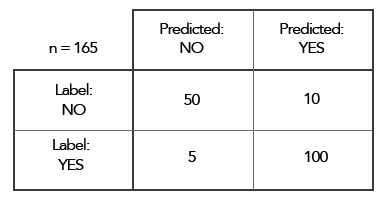
\includegraphics[scale=0.6]{confusion-matrix}
		\caption{Example of confusion matrix}
		\label{fig:mesh6}
	\end{figure}

	As it own name describes, the output of this type of metric consists of a matrix which shows a complete evaluation of the model. By definition, an entry $i,j$ of the matrix denotes the amount of observations that belong to group $i$ but are predicted as group $j$ \cite{Scikit-learn}. For example, considering a binary classification problem in which there are two classes, YES and NO, for a test set composed by 165 samples, the matrix included in figure \ref{fig:mesh6} is obtained. 
	
	There are four groups that can be extracted from this matrix: True positives, the samples that are predicted as YES and that is in fact their true label, True Negatives, those cases that were predicted as NO and they are originally labelled as NO, False Positives, in which the predicted label is YES but they are actually negative, and False Negatives, those in which the predicted label is NO when their original label is YES.
	
	This metric an the one explained before, accuracy, can be related by taking the diagonal of the matrix and computing the next operation:
	
	\[
	\ \ acc = \frac{TruePositives +\ FalseNegatives}{Total\ number\ of\ samples} = 
	\ \ \frac{100 +\ 50}{165} = 0.91
	\]
	
	When the classification task consists on more than two classes, a multiclass problem, a similar definition of the confusion matrix can be extended from the binary problem. Considering a certain observation $C_k$, the True positive part of the matrix is placed in the exact point where the column and the row of this certain observation are crossed, i.e, when the predicted label is equal to the true label. The False positives samples are placed along the column $C_k$ for all the rows $C_0, ..., C_{k-1}, C{k+1}, ..., C_n$ which refers to all the samples that have been misclassified with the class $C_k$. The False negatives are, however, all the samples that originally are labelled with $C_k$ tag but have been wrongly categorized with $C_0, ..., C_{k-1}, C{k+1}, ..., C_n$ classes. Finally, the True negative samples are distributed across all the other positions in the matrix. In figure \ref{fig:mesh9}, a good example for this explanation is shown.
	
	\begin{figure}[h]
		\centering
		\captionsetup{justification=centering}
		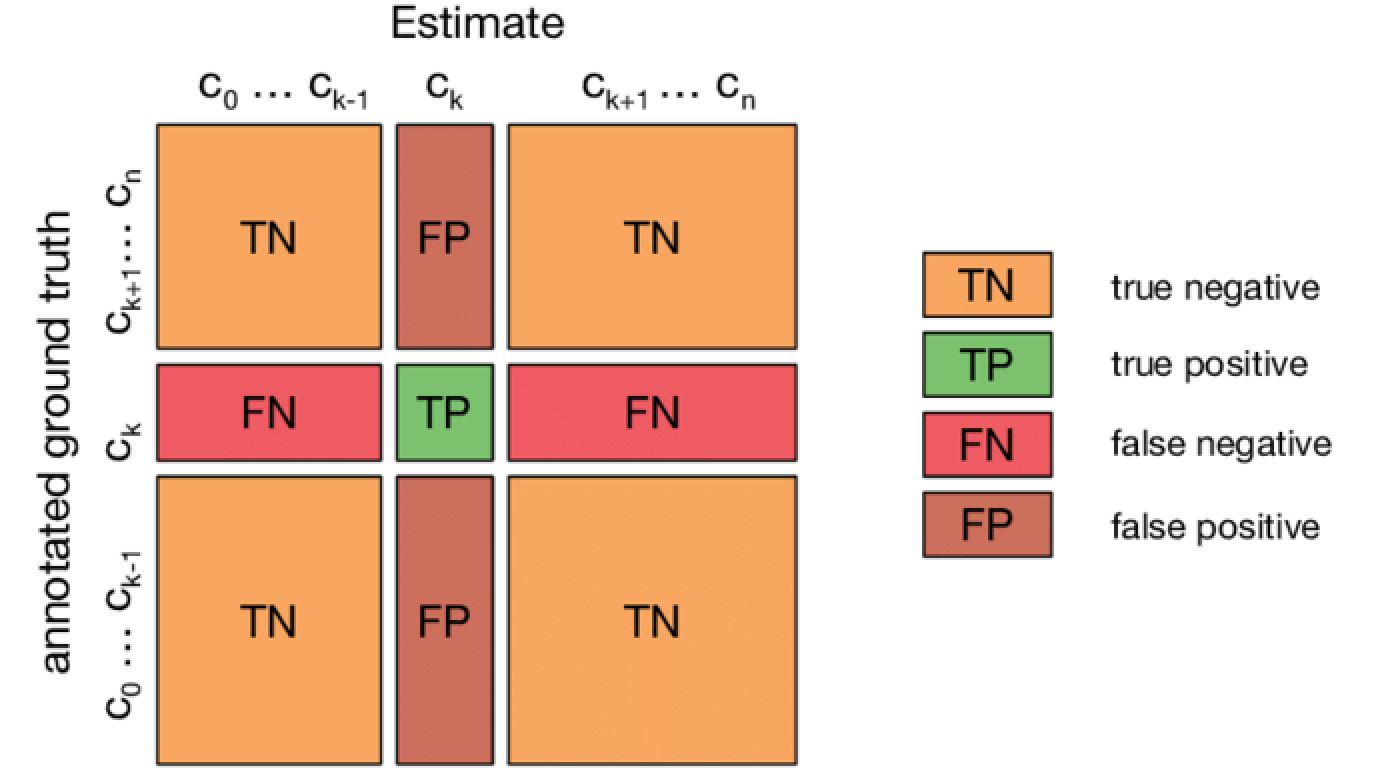
\includegraphics[scale=0.4]{conf-mat-multi}
		\caption{Confusion matrix for a multiclass classification \cite{Kruger2018}}
		\label{fig:mesh9}
	\end{figure}
	
\section{\acrlong{kfold}}
\label{appendix:kfold}

	The cross-validation technique consists in a resampling practice that is commonly used in order to evaluate machine learning algorithms when the dataset is not very large. It just depends on the parameter $k$ which represents the amount of folds or groups the data is going to be split into. This is the reason of the k-fold prefix. When the method is referred to in a situation in which the parameter is already fixed, for example, if $k = 5$, it can becomes named as 5-fold cross-validation.
	
	The purpose of this procedure is to check the performance of a machine learning model on unseen data. This is for not evaluating with the data used for the training process. It is really used nowadays and allows to obtain a less biased estimation than if using other kind of techniques as just a simple train and test split \cite{Browniee2018}. The steps followed by the method are listed below \cite{M2018}.
	
	\begin{enumerate}
		\item The data is split in a random way into $k$ folds. The value of this parameter can be chosen previously by running the algorithm for different options and picking the one with the best performance. However, a not very high value is usually chosen, keeping it in a range between 5 and 10.
		\item Fit the model by using the data in the $k - 1$ folds as train set, and the other part in the $k$ fold for the validation process. Collect the results for this configuration.
		\item The process must be repeated until all folds have been used as the validation set. Then, the average and standard deviation of all the results can be computed as the metric of the model. 
	\end{enumerate}

	Sometimes, instead of dividing the whole set of data in $k$ folds, it is first done a split into train and test sets. Then, the test set is excluded for a final measure and the train is split again with the \acrlong{kfold} procedure. The concept of the technique is shown in figure \ref{fig:mesh16}.
	
	\begin{figure}[ht]
		\centering
		\captionsetup{justification=centering}
		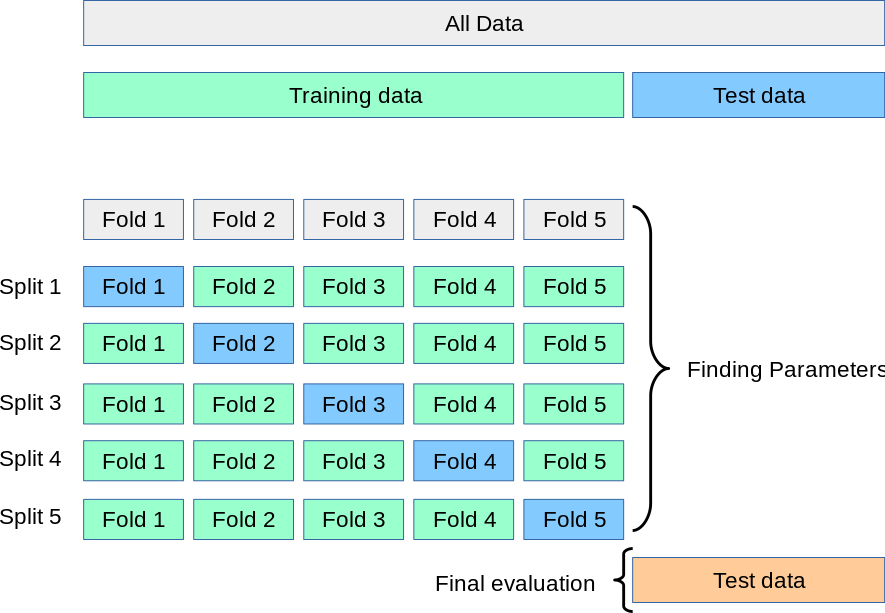
\includegraphics[scale=0.35]{k-fold}
		\caption{K-fold cross-validation scheme. The data is first split into train and test, and then the train is split again with this method \cite{Scikit-learna}}
		\label{fig:mesh16}
	\end{figure}

\section{Categorical cross-entropy}
\label{appendix:categorical-cross-entropy}

	In order to define this kind of loss function, it is necessary to consider the \textit{softmax} definition. As it was already explained in \ref{section:cnn}, this function takes a vector and represent its elements in the range (0,1) as probabilities, so all of the resulting values must sum up 1. In a multiclass classification, these are interpreted as class probabilities.
	
	These output probabilities can be evaluated with the cross-entropy loss. This is a way of measuring the performance of a model in which the output are probabilities between 0 and 1. The loss increases if the probability differs largely from the actual value of the true label. A perfect system would have a loss value of 0 \cite{MLGlossary2017}. In figure \ref{fig:mesh26}, it is shown an example of the loss function when the true label is 1.
	
	\begin{figure}
		\centering
		\captionsetup{justification=centering}
		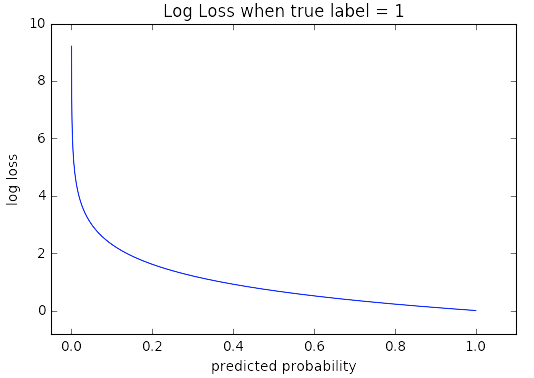
\includegraphics[scale=0.6]{ce}
		\caption{Cross-entropy loss function when the true label is equals to 1. As the probability of the predicted class approaches to 1, the loss function tends to zero. However, if it the probability is closer to 0.0, then the loss function increases heavily \cite{MLGlossary2017}.}
	\end{figure}

	Its formula is defined for binary problems as follows:
	
	\[
	\ CE = -(ylog(p) + (1 - y)log(1 - p))
	\]

	For a multiclass case, a unique loss is computed for each class label for each sample, and then add the results as follows:
	
	\[
	\ CE = - \sum_{c=1}^{M} y_{o,c}log(p_{o,c})
	\]
	
	Where $M$ is then number of classes, $y$ is a indication in binary format if the class $c$ is the right prediction for this sample $o$ and $p$ is the estimation probability of $c$ for $o$ \cite{MLGlossary2017}. 
	
	Then, the categorical cross-entropy is a combination of softmax and the cross-entropy loss.
	
	
	